\documentclass{article}
\usepackage[tmargin=1in, bmargin=1in, lmargin=1.5in, rmargin=1.5in]{geometry}
\usepackage[MeX]{polski}
\usepackage[utf8]{inputenc}
\usepackage{array}
\usepackage{longtable}
\usepackage{pdfpages}

\newcolumntype{L}[1]{>{\raggedright\let\newline\\\arraybackslash\hspace{0pt}}m{#1}}
\newcolumntype{C}[1]{>{\centering\let\newline\\\arraybackslash\hspace{0pt}}m{#1}}
\newcolumntype{R}[1]{>{\raggedleft\let\newline\\\arraybackslash\hspace{0pt}}m{#1}}


\author{Fundacja nowoczesna szkoła\\\\
Honorata Rosłanowska \\
Marcin Wardziński\\
Kacper Sarnacki \\
Łukasz Dragan \\
Kacper Trojanowski \\
Mateusz Flis \\
Michał Grabowski \\
Piotr Waszkiewicz}
\title{System polis ubezpieczeniowych}

\begin{document}
\maketitle
\newpage
\tableofcontents
\newpage

\section{Interesariusze}
\def\arraystretch{2.3}
\setlength\LTleft{-2.5cm}
\begin{longtable}{|l|L{0.2\textwidth}|L{0.58\textwidth}|C{0.15\textwidth}|C{0.15\textwidth}|}
\hline
\textbf{Kategoria} & \textbf{Interesariusz} & \textbf{Rola} & \textbf{Wpływ na projekt} & \textbf{Zaangażowanie} \\ \hline
Wewnętrzni & Sponsor PW & ponosi odpowiedzialność za projekt, jest decyzyjny w sprawach budżetu oraz odpowiada za negocjacje z klientem. Może wnioskować o zmianę budżetu, może zwalniać i zatrudniać pracowników, odpowiada za projekt. & 2 & 0 \\ \hline
 & PM ŁD & może wnioskować o zmianę budżetu, może zwalniać lub zatrudniać pracowników, odpowiada za realizację projektu & 2 & 2 \\ \hline
 & Programiści & odpowiadają za realizację zadań, mogą wnioskować o modyfikację zakresu zadań, mogą wstrzymywać realizację zadań, mogą wnioskować o zmianę harmonogramu, & 1 & 1 \\ \hline
 & Specjaliści do spraw UX & odpowiadają za projektowanie interfejsu, prowadzą testy interfejsu, mogą modyfikować układ interfejsu & 1 & 1 \\ \hline
 & Specjalista ds. integracji HR & odpowiada za zarządzanie dostępem i uprawnieniami użytkowników, odpowiada za przeprowadzenie skutecznej integracji systemów, & 1 & 0 \\ \hline
 & Specjalista ds. baz danych KS & odpowiada za tworzenie i aktualizację baz danych, jest odpowiedzialny za skuteczną migrację baz danych & 1 & -1 \\ \hline
 & Analityk systemowy MW & opracowuje schemat logiczny działania systemu & 2 & 1 \\ \hline
 & Testerzy & są odpowiedzialni za testy funkcjonowania systemu, testy użyteczności interfejsu, sporządzanie raportów z przeprowadzonych testów & 0 & 1 \\ \hline
 & Specjalista ds. wdrożeń KT & jest odpowiedzialny za wdrożenie systemu, przeniesienie ze środowiska developerskiego do środowiska produkcyjnego & 0 & -2 \\ \hline
 & Specjaliści ds. szkoleniowych & są odpowiedzialni za przeszkolenie użytkowników na poszczególnych poziomach i za dostosowanie kompetencji personelu do właściwych, przypisanych im ról w systemie & -1 & -1 \\ \hline
 & Dyrektor finansowy AB & jest odpowiedzialny za zarządzanie realizacją budżetu i kontrolowanie ponoszonych wydatków & 2 & -1 \\ \hline
Zewnętrzni & Kierownik PW & może zmieniać budżet, może anulować projekt, może zmieniać harmonogram, odpowiada za negocjacje & 1 & 0 \\ \hline
 & Administratorzy poprzedniego systemu & są odpowiedzialni za zarządzanie istniejącym systemem & 0 & -2 \\ \hline
 & Agenci ubezpieczeniowi & korzystają z systemu w roli zaawansowanych użytkowników & 2 & 2 \\ \hline
 & Użytkownicy & wykorzystują system do zakupu polis ubezpieczeniowych & -1 & -1 \\ \hline
 & Product Owner DC & jest odpowiedzialny za utrzymanie i ewentualne modyfikacje ostatecznych funkcjonalności systemu, wspiera analityka systemowego & 2 & 1 \\ \hline
 & Księgowi & posiadają szczegółową wiedzę z zakresu logiki systemu, lecz jego wdrożenie zredukuje liczbę miejsc pracy & 2 & -2 \\ \hline
\end{longtable}

\begin{figure}[h]
    \centering
    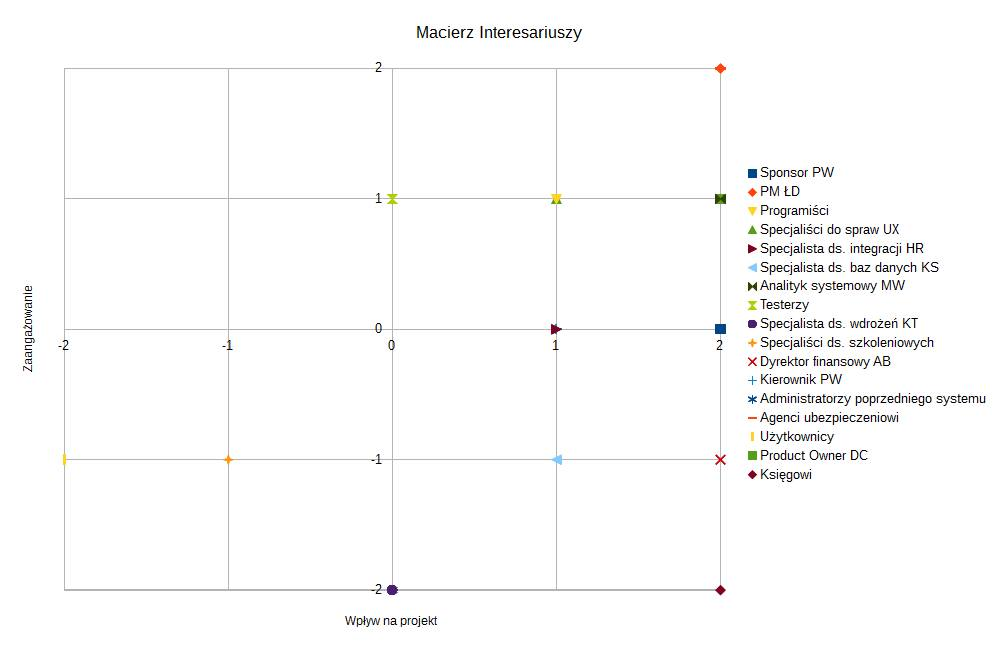
\includegraphics[scale=0.4]{macierz_interesariuszy.png}
    \caption{Macierz interesariuszy}
\end{figure}


\section{Zasady komunikacji}
\begin{enumerate}
	\item Komunikacja w projekcie pomiędzy Zamawiającym a Wykonawcą odbywać się będzie na niżej
	wymienionych poziomach:
	\begin{itemize}
		\item Kierownik projektu PW - Menadżer zespołu developerskiego Wykonawcy ŁD
		\item Product Owner DC  - Analityk systemowy Wykonawcy MW
		\item Agenci ubezpieczeniowi - Analityk systemowy Wykonawcy MW
		\item Księgowi - Analityk systemowy Wykonawcy MW
		\item Administratorzy poprzedniego systemu - zespół developerów Wykonawcy
	\end{itemize}
	\item Wszelkie przekazywane przez Zamawiającego produkty (w tym wszystkie dokumenty)
	przekazywane są również do repozytorium projektu. Do czasu uruchomienia repozytorium
	projektu dokumenty będą przekazywane na adres. repozytorium@company.com %TODO czy wykonawca czy zamawiający?
	\item Wszystkie spotkania między Zamawiającym a Wykonawcą będą protokołowane (zgodnie z szablonem Protokół ze Spotkania) %TODO załączniki uwzględniać?
	oraz wysyłane do Zamawiającego. Brak uwag lub ich nie przesłanie w uzgodnionym terminie jest uznawany za akceptację protokołu przez
	uczestników spotkania.
	\item W wyniku spotkań analitycznych mogą powstać zebrane wymagania – w rejestrze wymagań,
	z którego wyciąg jest załączany do Protokołu ze Spotkania.
	\item W przypadku, gdy osoba korzystająca z repozytorium zauważy, że ma dostęp do innych
	zasobów, niż te, do których powinna mieć dostęp, musi niezwłocznie poinformować o tym
	menadżera projektu ŁD.
	\item Niezależnie od postanowień Umowy zobowiązującej do przedstawienia określonych
	dokumentów w formie pisemnej wszelkie oficjalne zawiadomienia, zapytania lub
	informacje odnoszące się lub wynikające z wykonywania umowy wymagają formy pisemnej.
	Dopuszcza się stosowanie uzgodnień w formie poczty elektronicznej.
\end{enumerate}

\section{Metody komunikacji}
\begin{itemize}
	\item Spotkania - komunikacja bezpośrednia
	\item Raporty
	\item Poczta elektroniczna
	\item Szkolenia
	\item Rozmowy telefoniczne
	\item Repozytorium projektu
\end{itemize}

\subsection{Spotkania}
Spotkanie powinno być uzgadniane z co najmniej trzydniowym wyprzedzeniem. Wszystkie osoby uczestniczące w nim powinny dostać maila informującego o szczegółach: dacie, godzinie, miejscu i tematyce spotkania. Uczestnicy mają dzień na potwierdzenie udziału lub zgłoszenie ewentualnych uwag.

W każdym spotkaniu musi uczestniczyć osoba tworząca protokół ze spotkania. Ów protokół powinien zawierać czas i miejsce spotkania, uczestników oraz zagadnienia poruszone na spotkaniu, a także postanowienia. Protokół powinien być wgrany na repozytorium projektu nie później niż dwa dni po spotkaniu.

\subsection{Raporty}
Raport ze spotkania powinien zawierać informację o spotkaniu, z którego jest tworzony oraz o jego dacie i miejscu. Powinien zawierać informacje o przebiegu spotkania oraz wnioski, które zostały wyciągnięte w trakcie jego trwania. Raport powinien zostać dostarczony pocztą elektroniczną. 

Pisemny raport z postępów prac powinien zawierać przedział czasowy, w którym prace były wykonywane oraz wypunktowane zadania, które zostały wykonane. Powinien zostać dostarczony pocztą elektroniczną.



\subsection{Poczta elektroniczna}
Osoba, tworząca nowy wątek, powinna nadać mu temat konkretny i wskazujący, czego dotyczy treść maila. 

Osoba odpowiadająca na maila powinna odpowiedzieć w tym samym wątku (nie tworzyć nowego). Musi wysłać maila do wszystkich osób uczestniczących w danym wątku, tj. nadawcy i wszystkich adresatów.

\subsection{Szkolenia}
Szkolenie powinno być uzgodnione z co najmniej tygodniowym wyprzedzeniem. Wszystkie osoby uczestniczące w nim powinny dostać maila informującego o szczegółach: dacie, godzinie, miejscu i tematyce spotkania. Uczestnicy mają dzień na potwierdzenie udziału lub zgłoszenie ewentualnych uwag.

W każdym szkoleniu musi uczestniczyć osoba tworząca protokół ze szkolenia. Ów protokół powinien zawierać czas i miejsce szkolenia, uczestników oraz zagadnienia poruszone na szkoleniu. Protokół powinien być wgrany na repozytorium projektu nie później niż dwa dni po szkoleniu.

\subsection{Rozmowy telefoniczne}
Wszystkie rozmowy telefoniczne w celach biznesowych powinny być nagrywane, za zgodą obu stron. Następnie na podstawie rozmów powinny być tworzone raporty, zawieające wnioski z rozmowy. Raport powinien być wgrany na repozytorium nie później niż dwa dni po rozmowie.

\subsection{Repozytorium}
Używanym repozytorium będzie BitBucket. Do zarządzania procesem tworzenia oprogramowania będzie służyć JIRA. Zadania reprezentowane będą przy pomocy Issues. Developer wybiera issue, które chce wykonać i tworzy w tym celu branch o nazwie \textit{feature/*} gdzie * to numer rozwiązywanego issue. Po skończonej pracy każda zmiana, przed mergem do głównego brancha powinna być zatwierdzona przez testera. Developer tworzący brancha jest odpowiedzialny za merge i rozwiązanie ewentualnych konfliktów.

\newpage
\section{Plan komunikacji}
\def\arraystretch{2.5}
\setlength\LTleft{-2.5cm}
	\begin{longtable}{|L{0.20\textwidth}|L{0.26\textwidth}|L{0.20\textwidth}|L{0.26\textwidth}|L{0.28\textwidth}|}
		\hline
		\textbf{Zainteresowane strony } & \textbf{Przekazywana informacja} & \textbf{Dostawca informacji} & \textbf{Częstotliwość} & \textbf{Metoda komunikacji} \\ \hline
		\endhead
		\multicolumn{ 5}{|c|}{\textbf{Wychodzące}} \\ \hline
		Kierownik PW & Raport z postępu prac & PM ŁD & Nie rzadziej niż co dwa tygodnie & Poczta elektroniczna \\ \hline
		Kierownik PW & Projekt dokumentacji systemu & PM ŁD & Nie później niż 08.04.2016 & Spotkanie oraz przesłanie Poczta elektroniczna \\ \hline
		Kierownik PW & Ostateczna wersja dokumentacji do zatwierdzenia  & PM ŁD & Nie później niż 15.04.2016 & Poczta elektroniczna \\ \hline
		Kierownik PW & Propozycja Planu realizacji Etapu I & PM ŁD & Nie później niż tydzień po rozpoczęciu projektu & Poczta elektroniczna \\ \hline
		Kierownik PW & Raport końcowy z Etapu I & PM ŁD & Po akceptacji dokumentacji, Nie później niż 15.04.2016 & Poczta elektroniczna \\ \hline
		Kierownik PW & Propozycja Planu realizacji Etapu II & PM ŁD & Nie później niż tydzień przed końcem etapu I & Poczta elektroniczna \\ \hline
		Kierownik PW & Raport końcowy z Etapu II & PM ŁD & Nie później niż 15.06.2016 & Poczta elektroniczna \\ \hline
		Kierownik PW & Przekazanie końcowej dokumentacji systemu w wersji edytowalnej
		& PM ŁD & Nie później niż 30.06.2016 & Poczta elektroniczna \\ \hline
		Kierownik PW & Propozycja Planu realizacji Etapu III & PM ŁD & Nie później niż tydzień przed końcem etapu II & Poczta elektroniczna \\ \hline
		Kierownik PW & Raport końcowy z Etapu III & PM ŁD & Nie później niż 30.06.2016 & Poczta elektroniczna \\ \hline
		Kierownik PW & Przekazanie kodów źródłowych wraz z komentarzami & PM ŁD & Nie później niż 30.06.2016 & Przekazanie plików za pomocą sftp udostępnionego przez zamawiającego oraz przesłanie informacji Poczta elektroniczna o przekazaniu plików
		
		\\ \hline
		Kierownik PW & Projekt dwóch wersji interfejsów użytkownika & Specjaliści do spraw UX,
		Analityk systemowy MW & Nie później niż 08.04.2016 & Spotkanie \\ \hline
		Analityk systemowy MW, Księgowi,
		Użytkownicy (Agenci ubezpieczeniowi) & 
		Przekazanie kursów e-learningowych dla uzytkowników systemu  & Specjaliści ds. szkoleniowych & Nie później niż 30.06.2016 & Przekazanie plików za pomocą sftp udostępnionego przez zamawiającego oraz przesłanie informacji Poczta elektroniczna o przekazaniu plików
		
		\\ \hline
		Kierownik PW, Product Owner DC & Konsultacje analityczne z zamawiającym & Analityk systemowy MW & Nie częściej niż 2 razy w tygodniu do momentu zakończenia Etapu I, póżniej w razie potrzeby & Spotkanie \\ \hline
		Użytkownicy (Agenci ubezpieczeniowi), Product Owner DC
		& Konsultacje analityczne z użytkownikami obecnie działającego systemu
		& Analityk systemowy MW & W razie potrzeby & Spotkanie \\ \hline
		Księgowi, Product Owner DC & Konsultacje analityczne z księgowymi (użytkownikami systemu WF-FaKir)
		& Analityk systemowy MW & W razie potrzeby & Spotkanie \\ \hline
		\multicolumn{ 5}{|c|}{\textbf{Przychodzące}} \\ \hline
		PM ŁD & Zgoda na rozpoczęcie Etapu II & Kierownik PW & Do 15.04.2016 & Poczta elektroniczna \\ \hline
		PM ŁD & Zgoda na rozpoczęcie Etapu III & Kierownik PW & Do 30.06.2016 & Poczta elektroniczna \\ \hline
		PM ŁD & Zgoda na zmianę osób wskazanych w ofercie & Kierownik PW & Wyłącznie w przypadkach losowych & Przekazanie pisemnej zgody \\ \hline
		Administratorzy  systemu & Zgłaszanie błędów gwarancyjnych & Użytkownicy & Przez okres trwania gwarancji, w zależności od potrzeb & Telefoniczna linia serwisowa z automatyczną rejestracją zgłoszeń lub ogólna linia telefoniczna Wykonawcy
		\\ \hline
		\multicolumn{ 5}{|c|}{\textbf{Wewnętrzne}} \\ \hline
		PM ŁD & Raport z postępu prac & Programiści, 
		Analityk systemowy MW & Dwa razy w tygodniu & Spotkanie \\ \hline
		PM ŁD, Specjalista ds. baz danych, ds. wdrożeń, Analityk,
		& Informacje dotyczące migracji danych & Kierownik PW, Administratorzy obecnego systemu
		& Po zakończeniu etapu II & Spotkanie \\ \hline
		PM ŁD & Raport wyników testów akceptacyjnych & Testerzy & 11.06.2016 & Poczta elektroniczna \\ \hline
		PM ŁD & Raport z wyników testów integracyjnych & Testerzy, Specjalista ds. wdrożeń KT, 
		Specjalista ds. integracji HR & 27.06.2016 & Poczta elektroniczna \\ \hline
	\end{longtable}
	
\eject \pdfpagewidth=17in \pdfpageheight=11in
\begin{figure}
 \centering 
 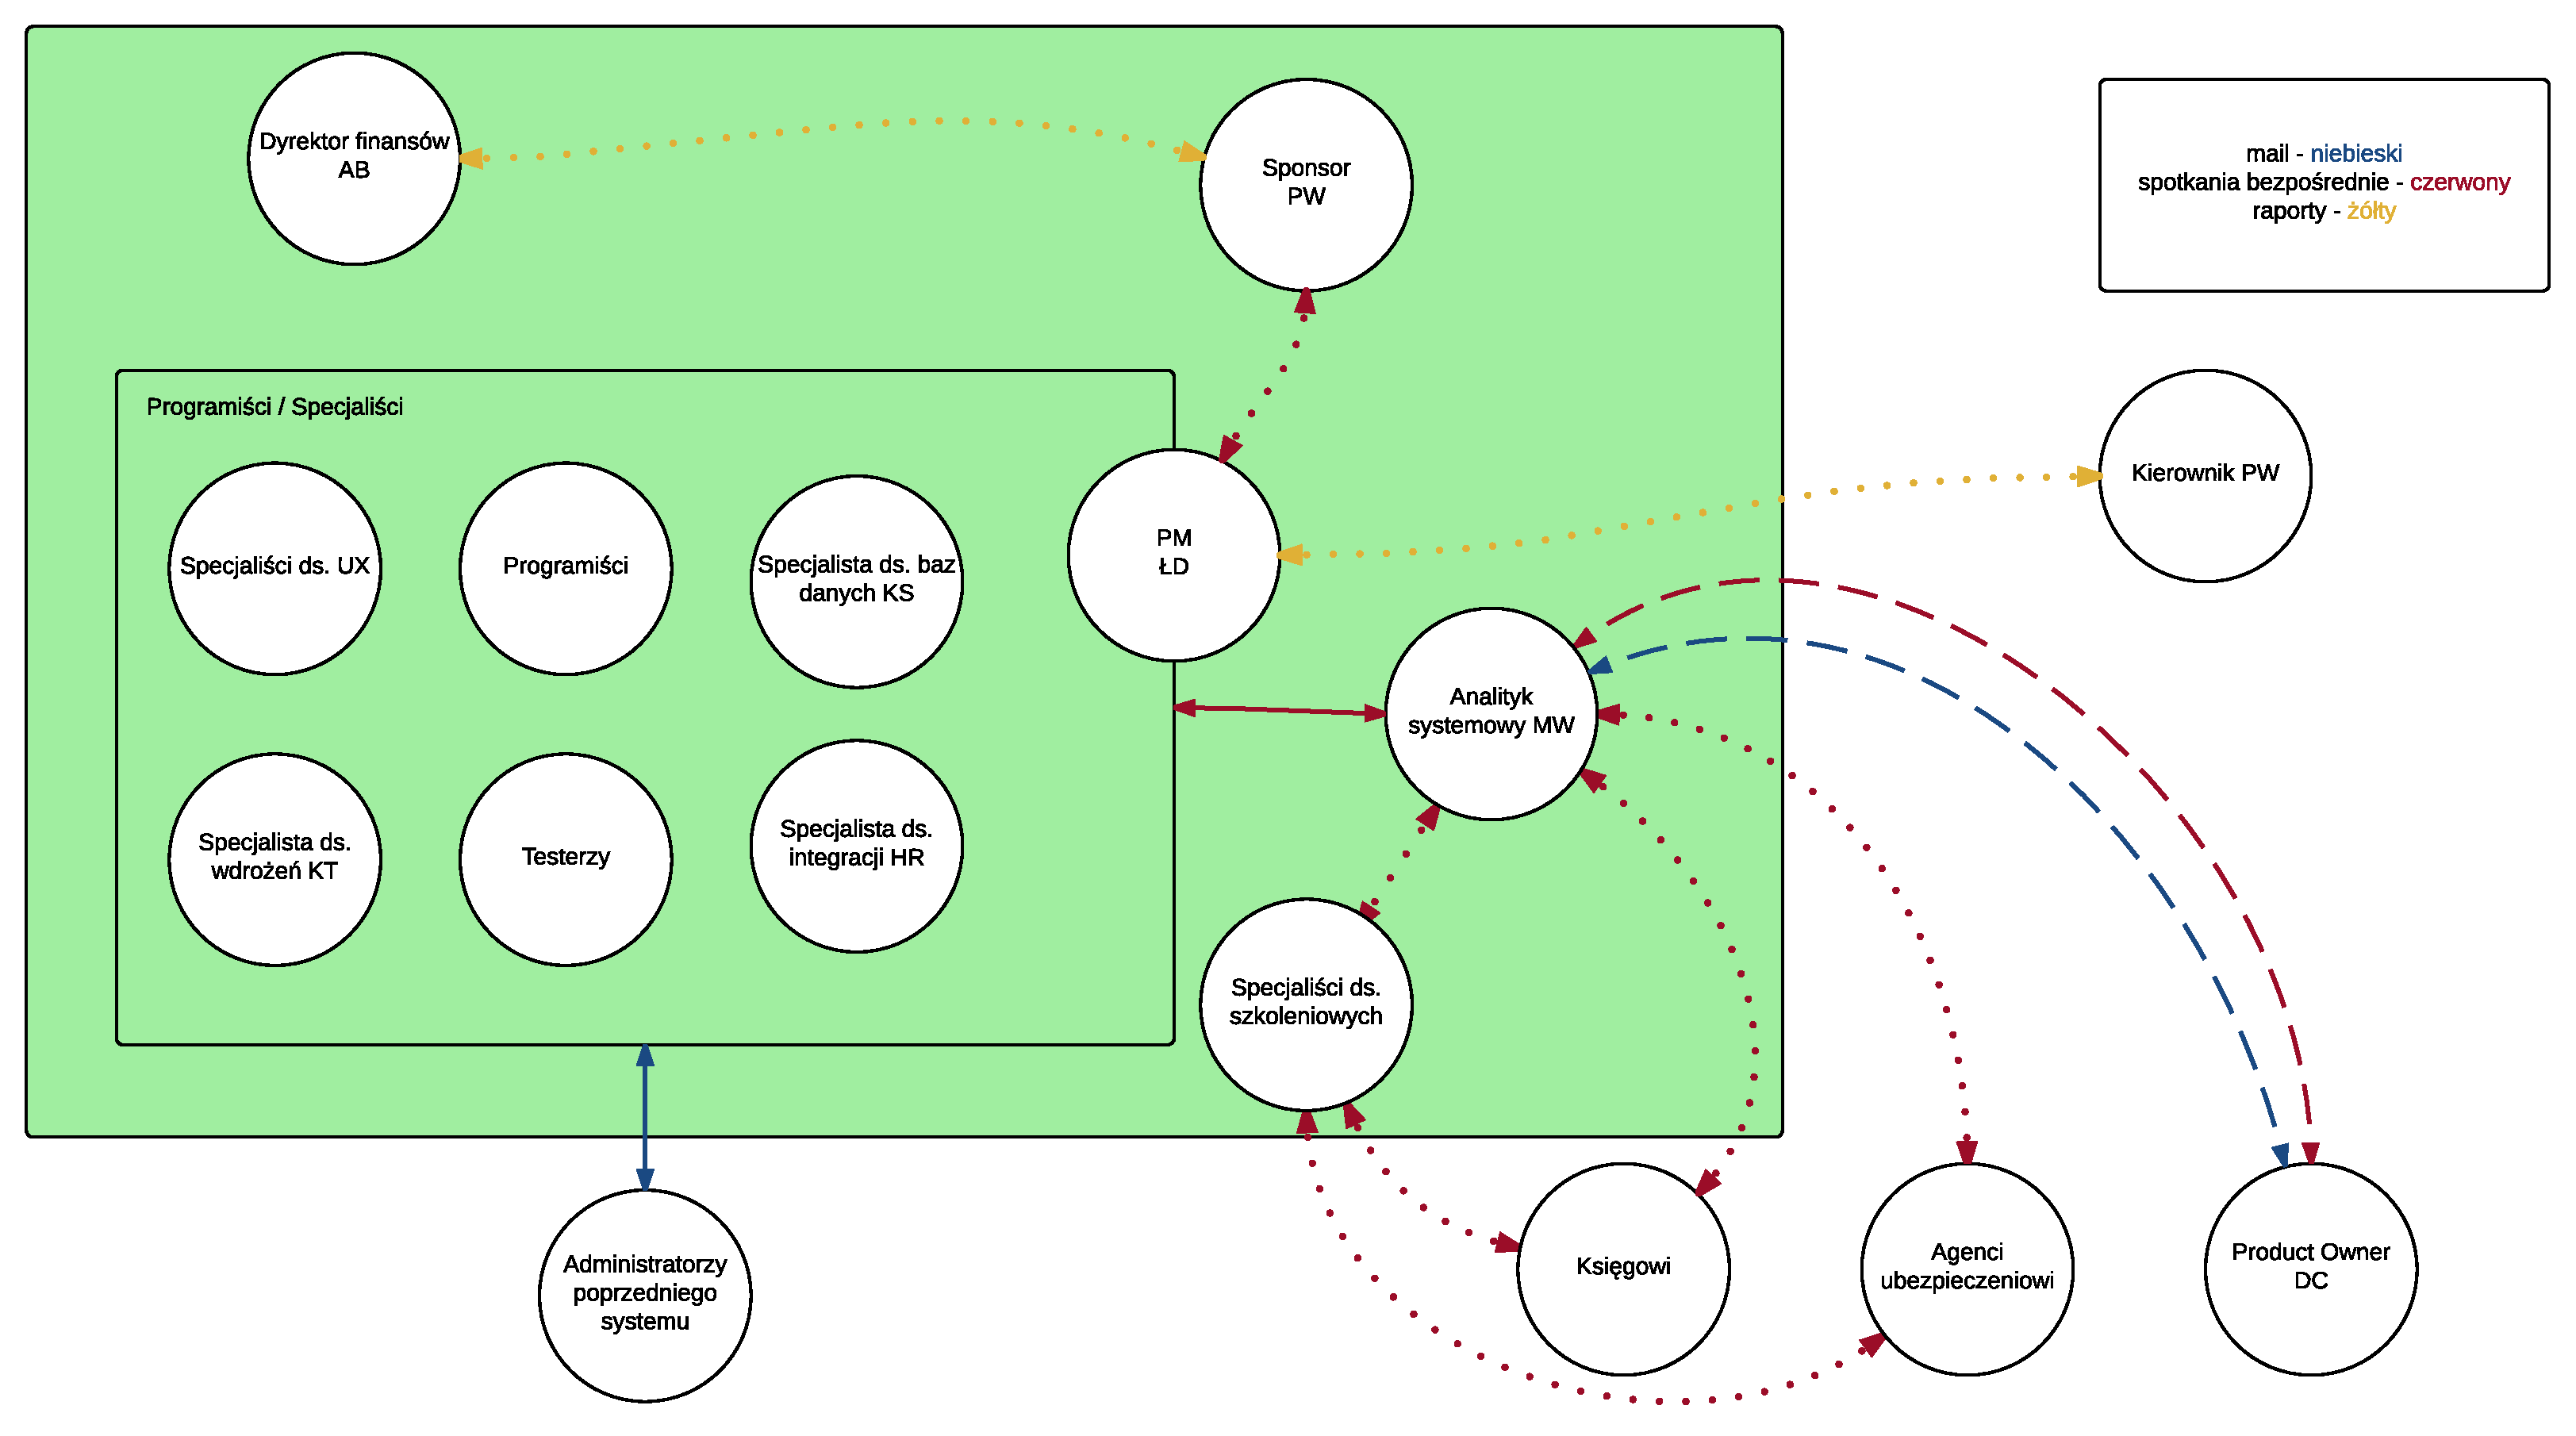
\includegraphics[scale=0.7]{komunikacja.pdf}
\end{figure}

\end{document}
